\newcommand{\figOverview}{%
  \begin{figure*}
    \centering
    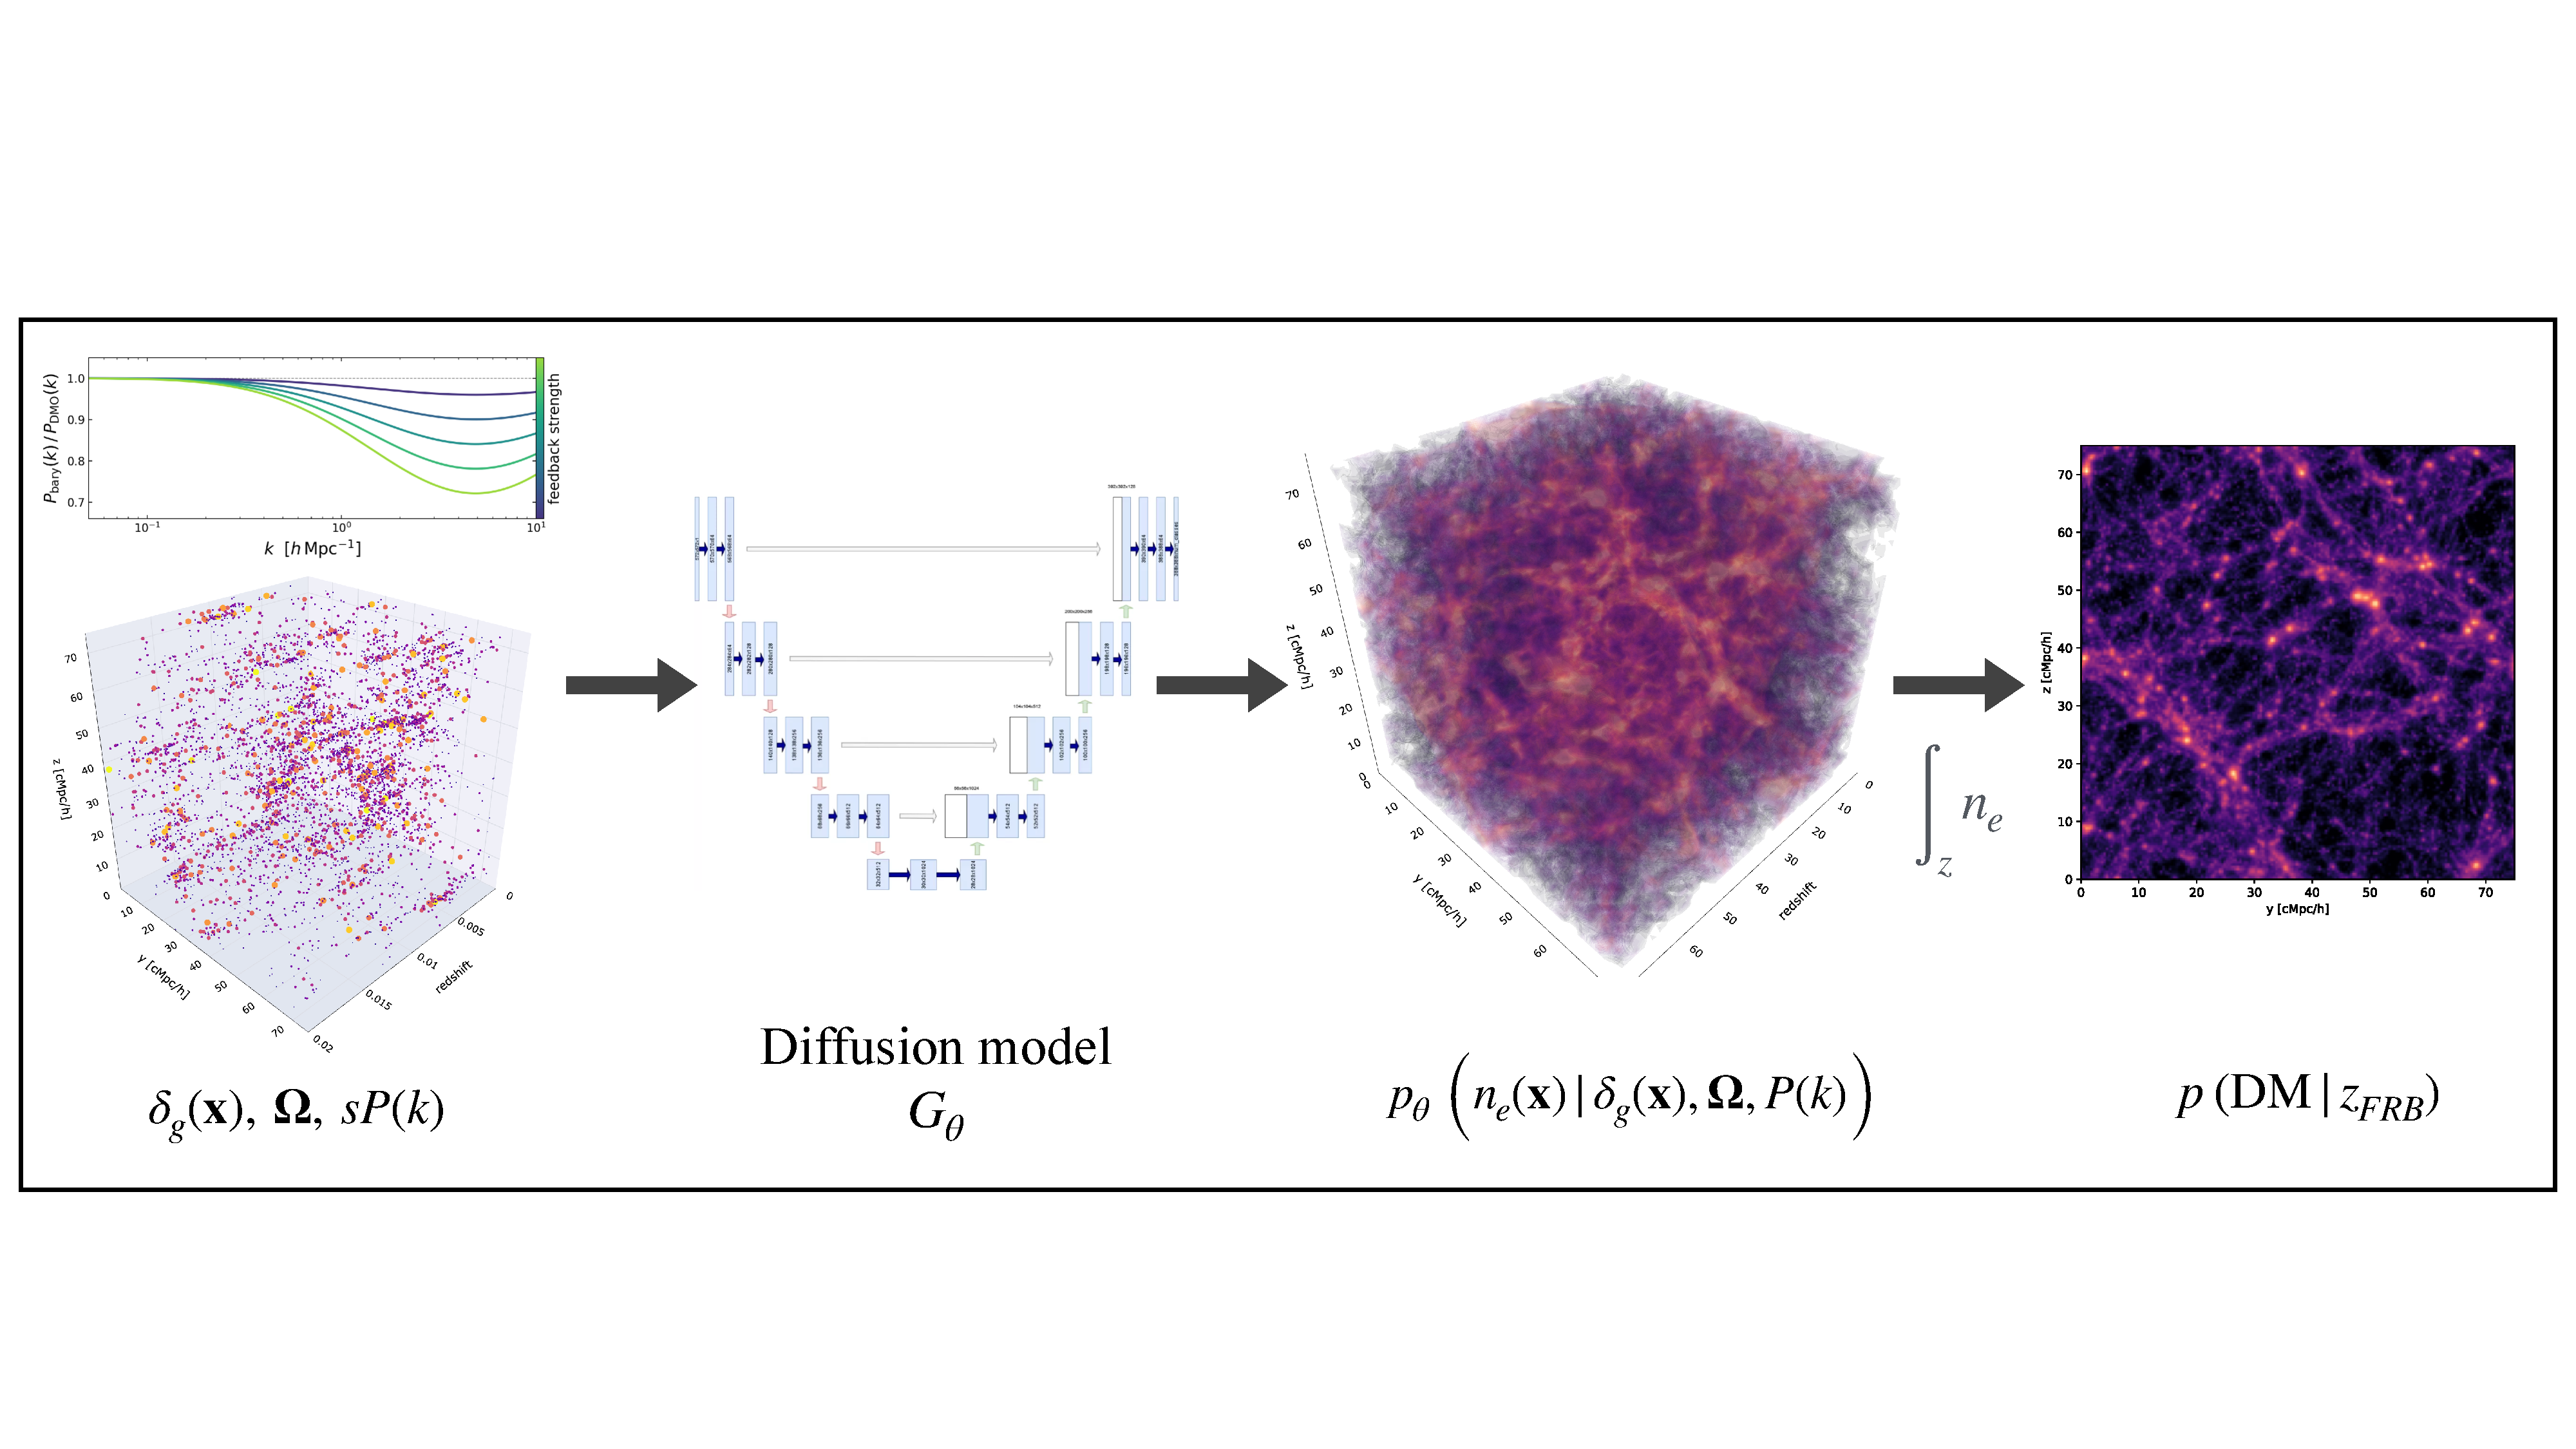
\includegraphics[width=\linewidth]{figures/DMDMfigure_maryam_paper.pdf}
    \caption{\textbf{Overview of our method for reconstructing the 3D distribution of cosmic baryons}: The diffusion model learns to recover the gas density field conditioned on input galaxy positions $\delta_g(\mathbf{x})$, the cosmological parameters $\mathbf{\Omega}$, and
    powerspectrum suppression, $sP(k)$. The output is a density field of free electrons, $n_e(\mathbf{x})$, which can
    be integrated to predict FRB dispersion measures. The model is probabilistic, allowing sampling from a reconstruction posterior.
    }
    \label{fig:overview-fig}
  \end{figure*}
}

\newcommand{\figInput}{%
  \begin{figure*}
    \centering
    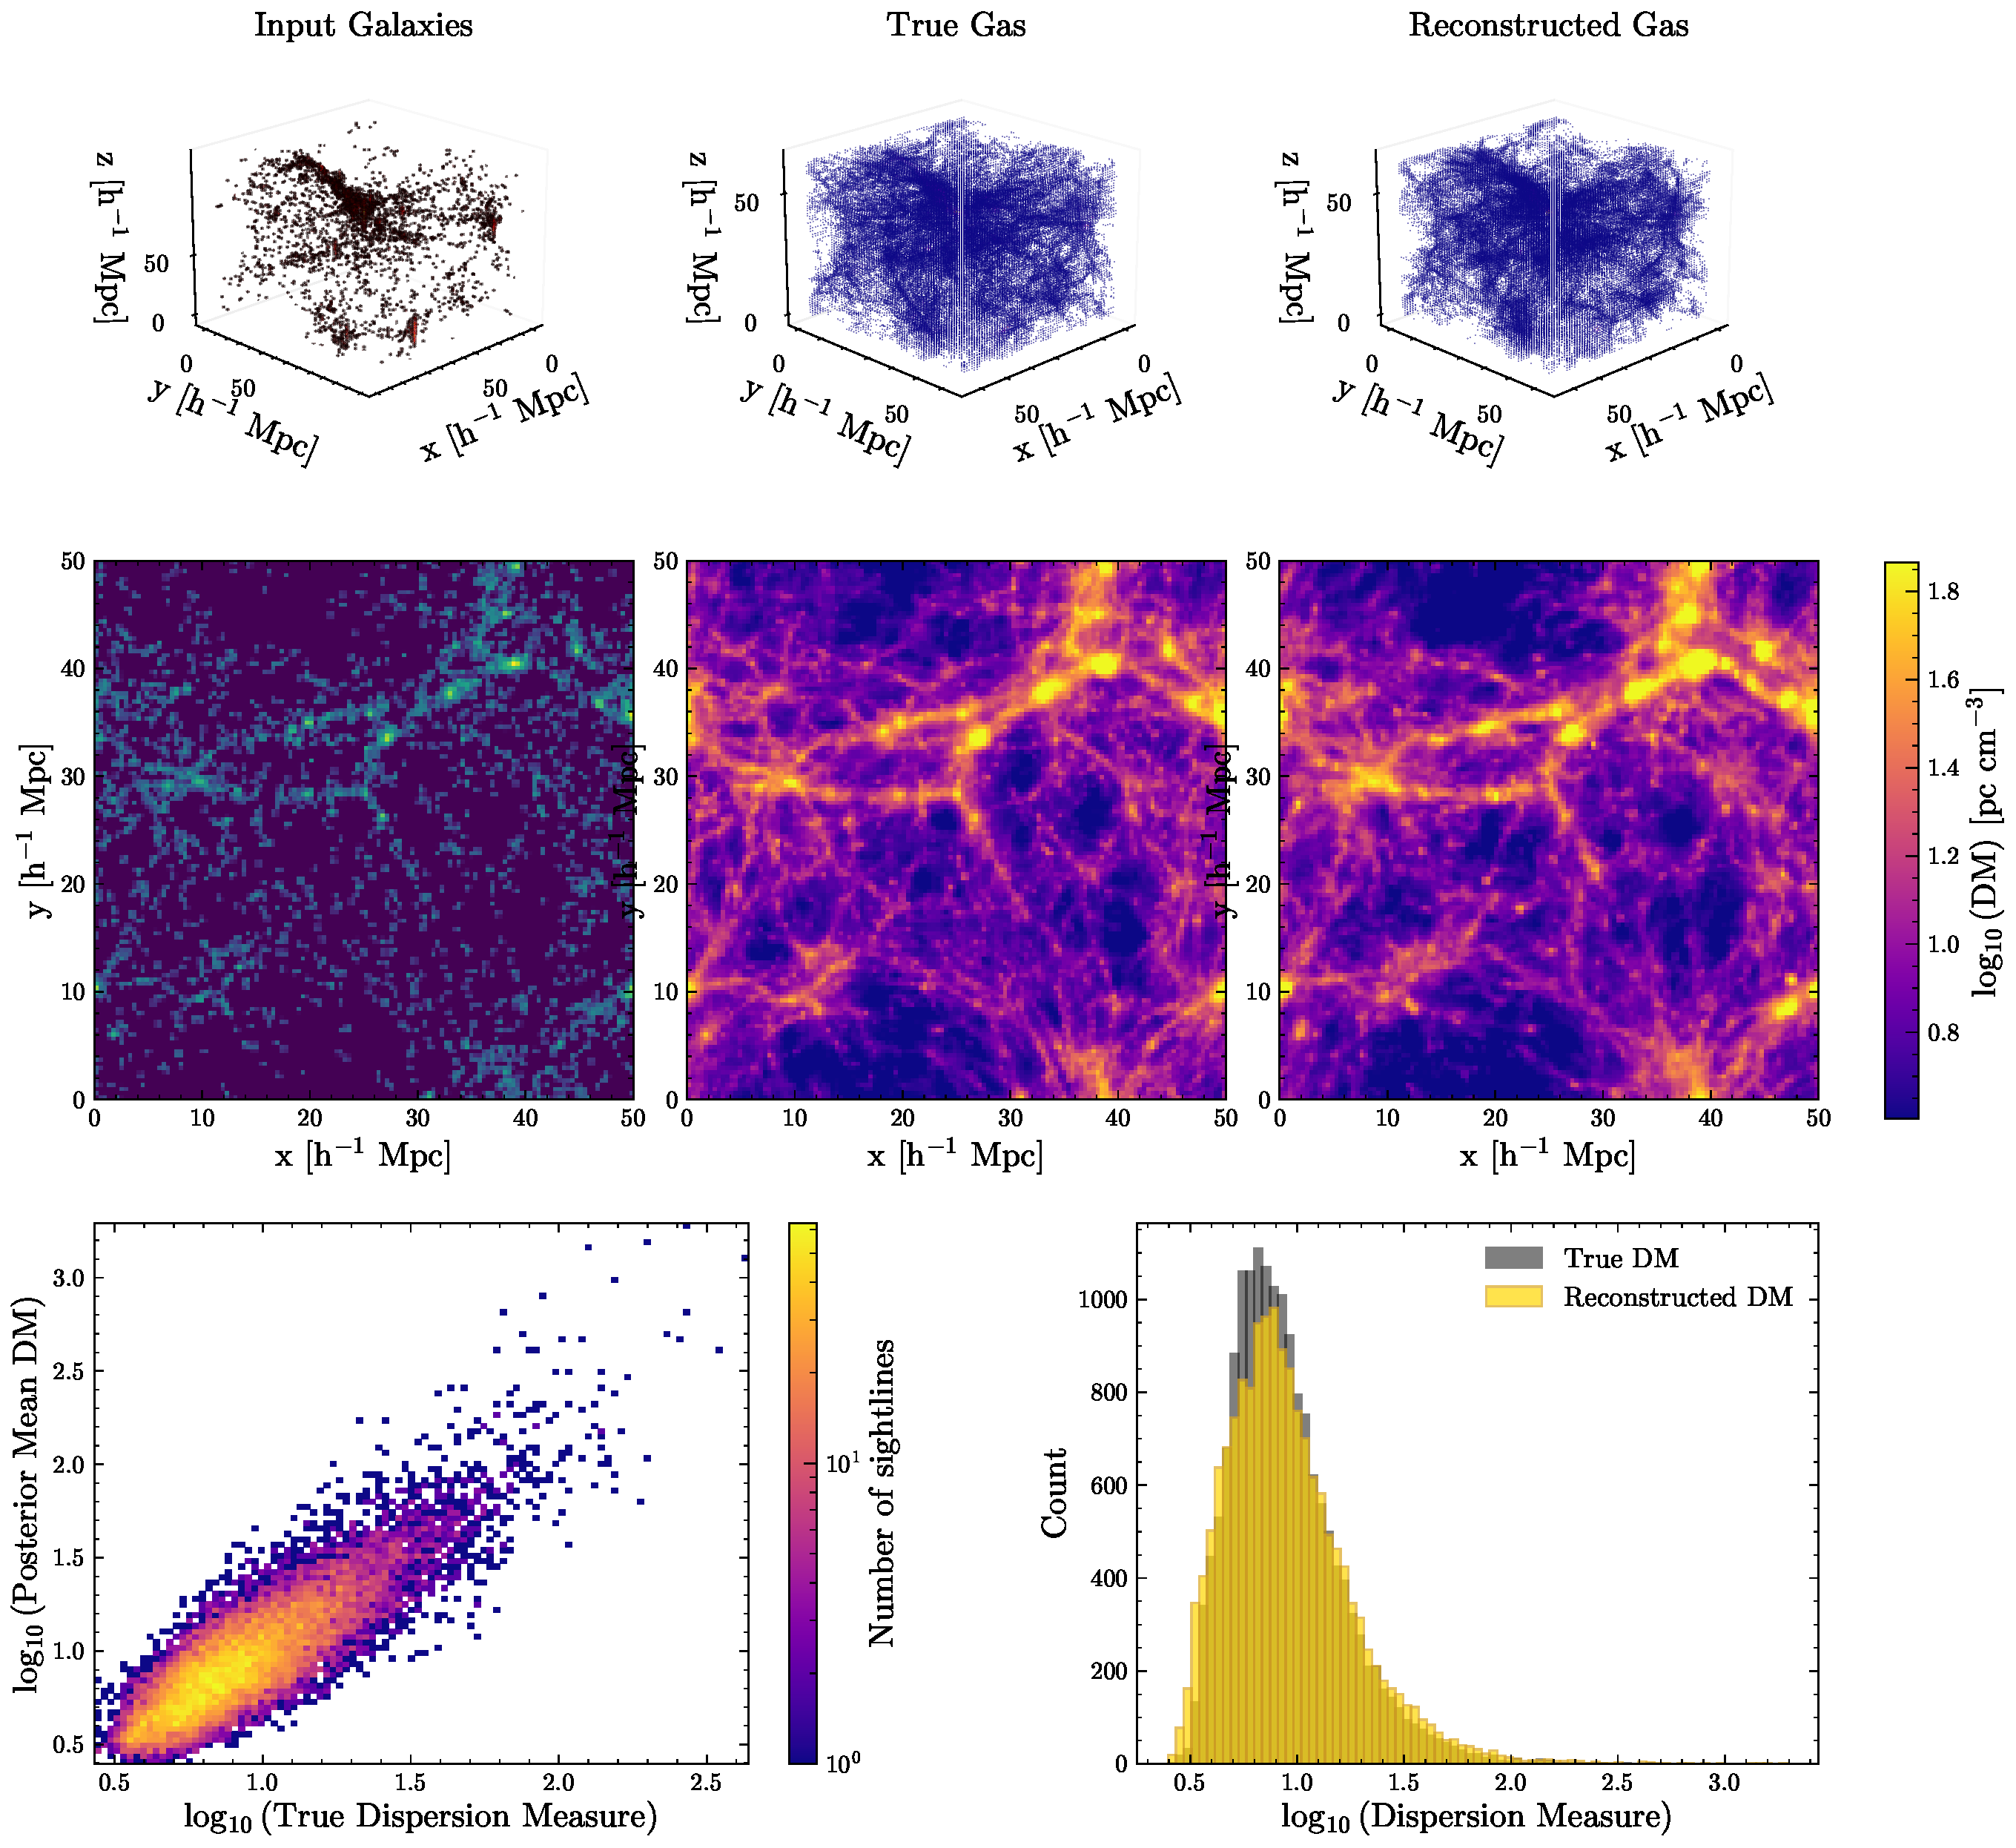
\includegraphics[width=0.98\linewidth]{figures/combined_3d_2d_histograms.pdf}
    \caption{\textbf{Top row:} Three-dimensional views of the input galaxy density field (left), true gas density from the simulation (center), and the model's reconstructed gas density (right), for a $(50\,h^{-1}\,\mathrm{Mpc})^3$ test box. \textbf{Middle row:} 2D maps of the input galaxy density field (left, projected along the line of sight), and the true and reconstructed dispersion measure (center and right) computed by summing gas density along the line of sight. \textbf{Bottom left:} 2D histogram plot of the model's posterior mean DM against the true DM across all pixels i.e lines of sight; the dashed line marks perfect 1:1 agreement. \textbf{Bottom right:} Histogram comparing the distribution of true DM values (gray) to reconstructed DM values (yellow). The model recovers both the spatial structure and the statistical distribution of the gas field.}
    \label{fig:input_output}
  \end{figure*}
}

\newcommand{\figPatchHist}{%
  \begin{figure*}
    \centering
    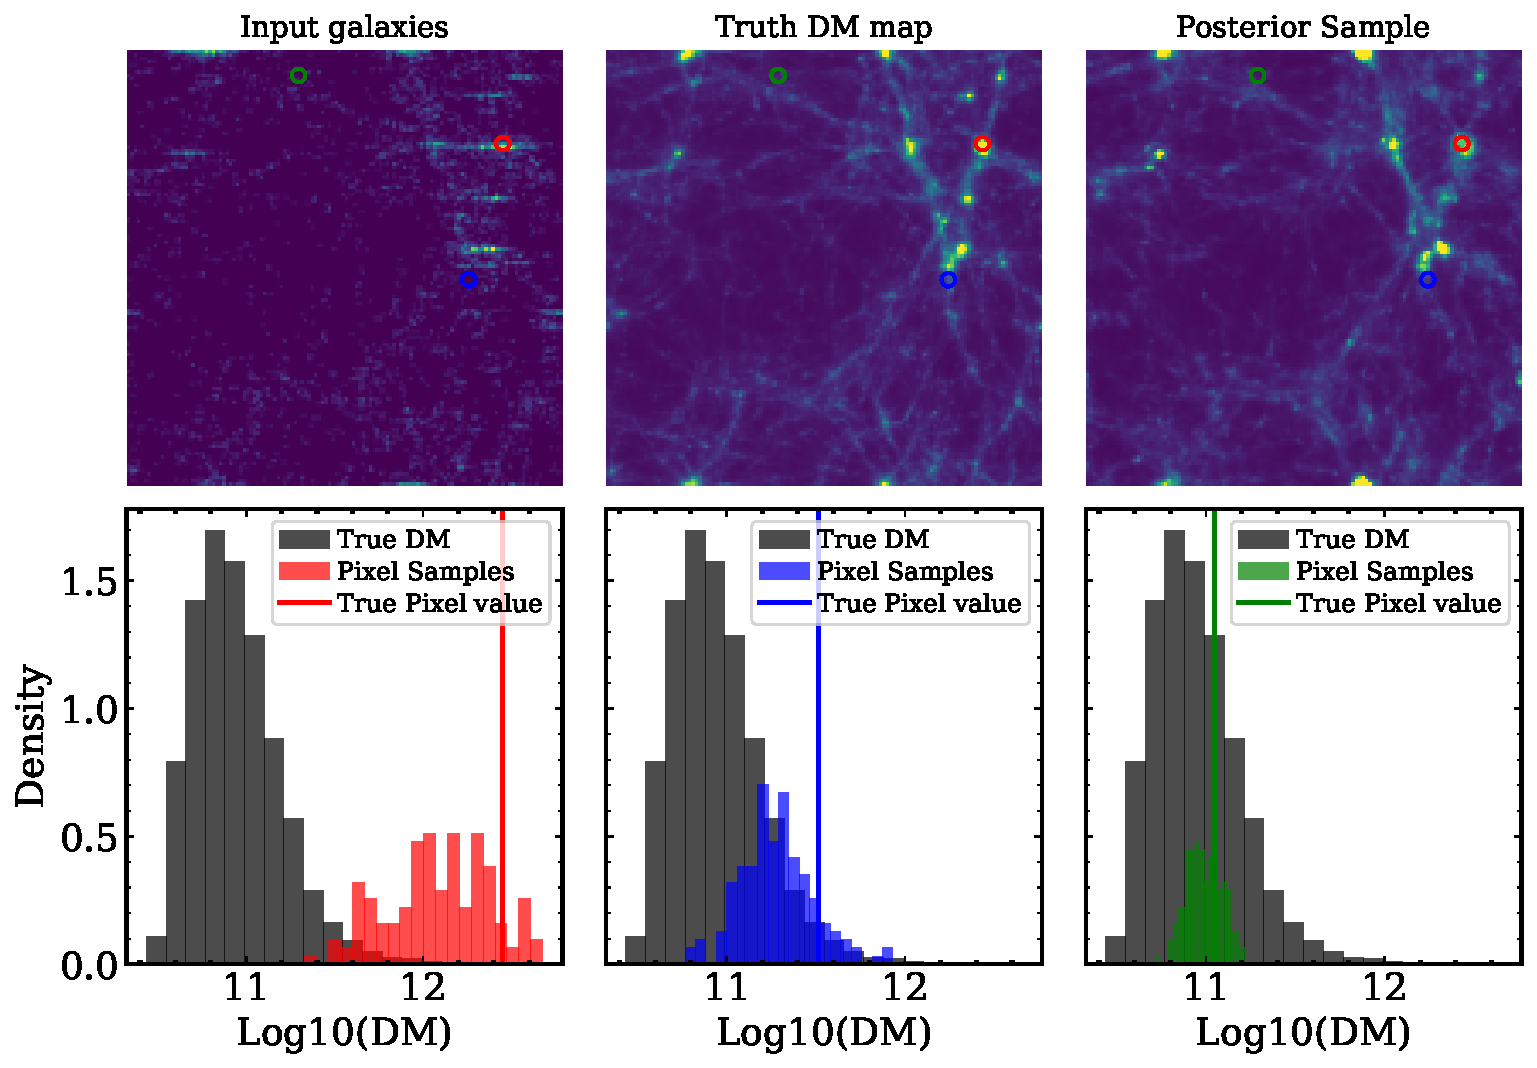
\includegraphics[width=0.5\linewidth]{figures/patch_hist_box9.pdf}
    \caption{\textbf{Top row, left to right:} Input galaxy density field and the true simulation DM map. \textbf{Bottom row, left to right:} The dispersion measure map of the model's posterior mean reconstruction; and the probability density of DM values at three representative sightlines marked in the maps spanning different cosmic environments (overdensity, moderate density, and underdensity). At each location, the colored distribution shows 150 independent posterior samples drawn from the diffusion model; the dashed vertical line marks the true DM value at that pixel; the gray distribution labeled ``True map'' shows the overall DM distribution across the full test box for reference. The model's posterior samples cluster tightly around the true DM value across all three environments, demonstrating well calibrated uncertainty estimates.}
    \label{fig:patch_hist_box9}
  \end{figure*}
}

\newcommand{\figFeedback}{%
  \begin{figure*}
    \centering
    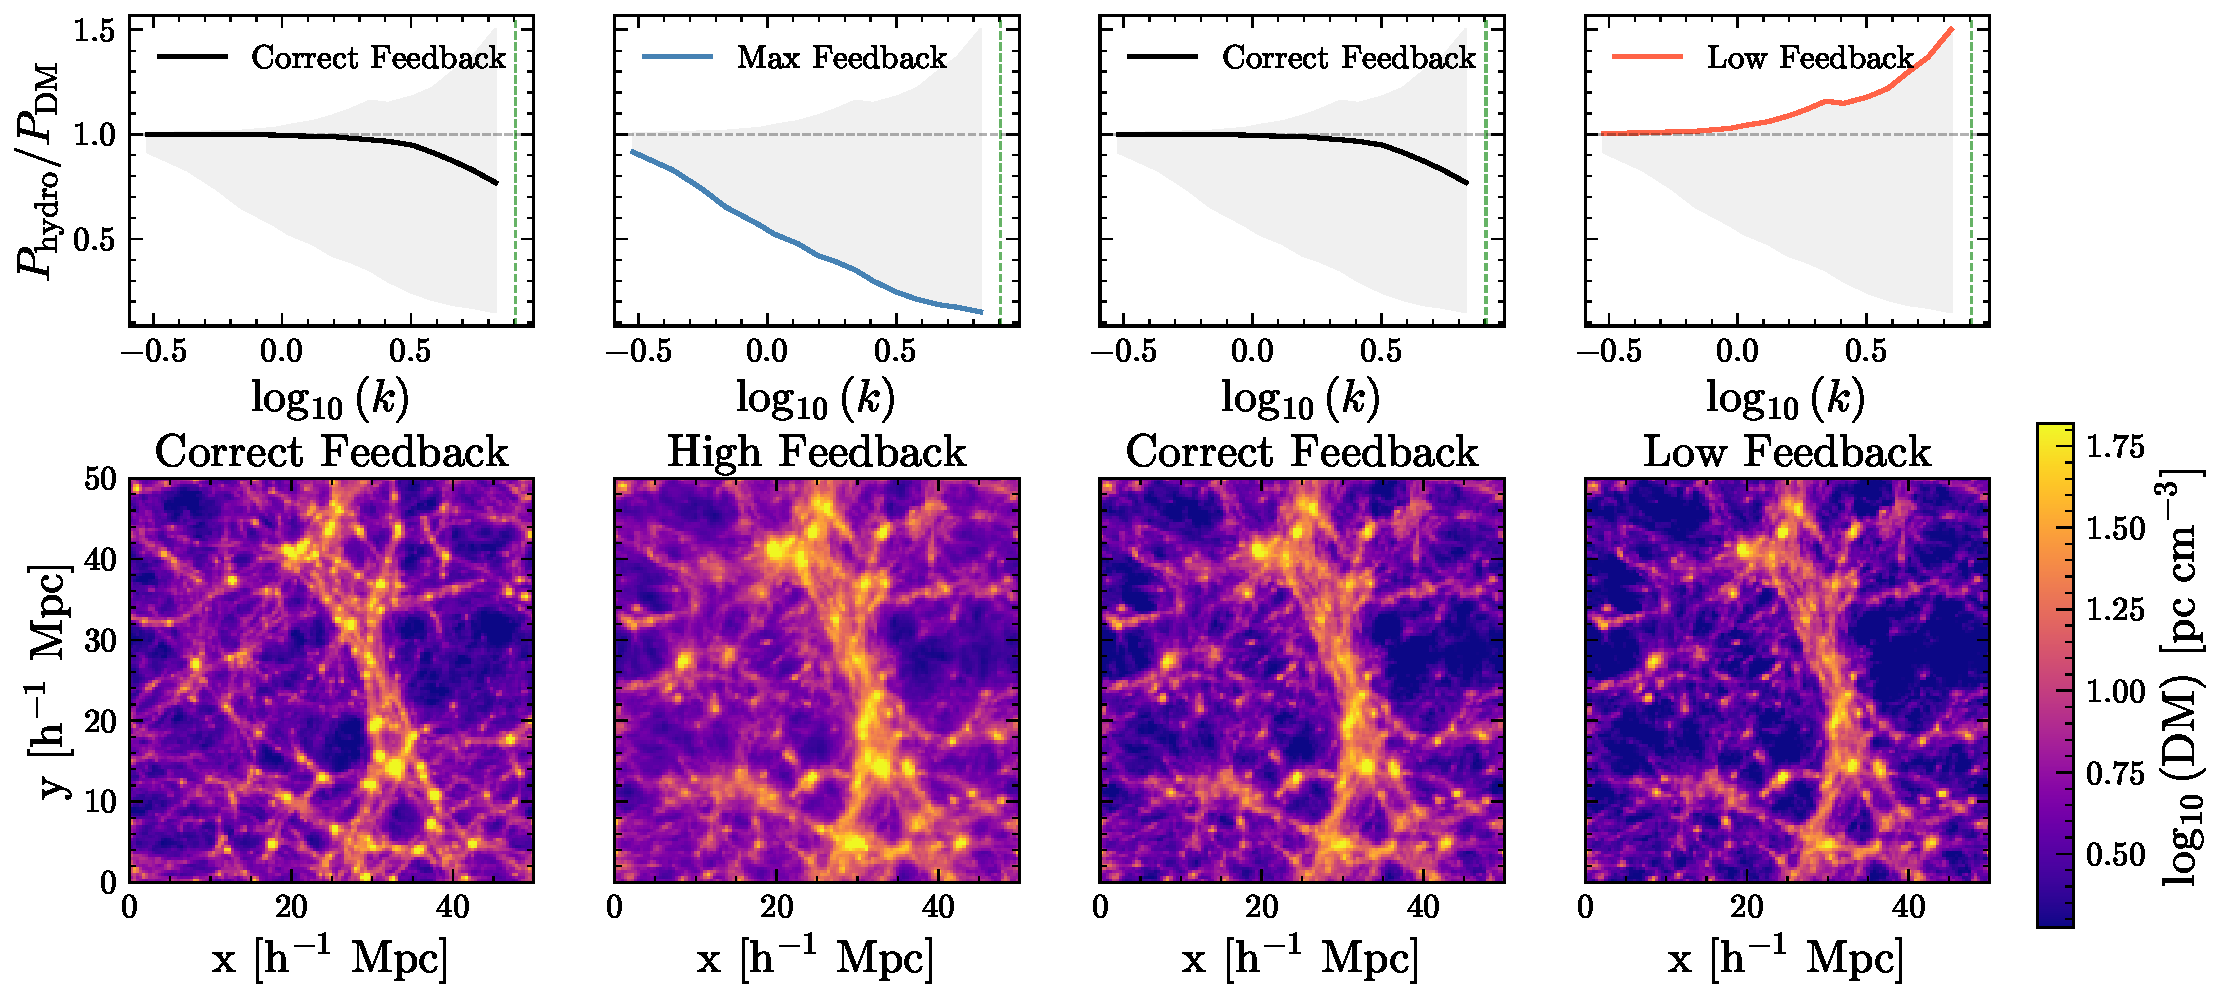
\includegraphics[width=0.95\linewidth]{figures/feedback_range.pdf}
    \caption{
        \textbf{Top row:} The baryon suppression spectrum $P_\mathrm{hydro}/P_\mathrm{DM}$ used to condition the model for four scenarios: maximum feedback, the true (correct) feedback matching the test box, and low feedback. \textbf{Bottom row:} Corresponding reconstructed DM maps for each conditioning scenario. The baryon suppression spectrum encodes both cosmological parameters (determining total baryon abundance) and feedback strength (determining baryon redistribution). At maximum feedback, the model predicts a more diffuse gas distribution reflecting strong feedback that expelled baryons from dense regions. At low feedback, the model predicts gas concentrated in filaments and nodes, consistent with higher baryon abundance and weaker feedback. The correct feedback panel matches the true field, validating that the model successfully learns the relationship between the suppression spectrum and gas structure.
    }
    \label{fig:pk}
  \end{figure*}
}

\newcommand{\figTNG}{%
  \begin{figure*}
    \centering
    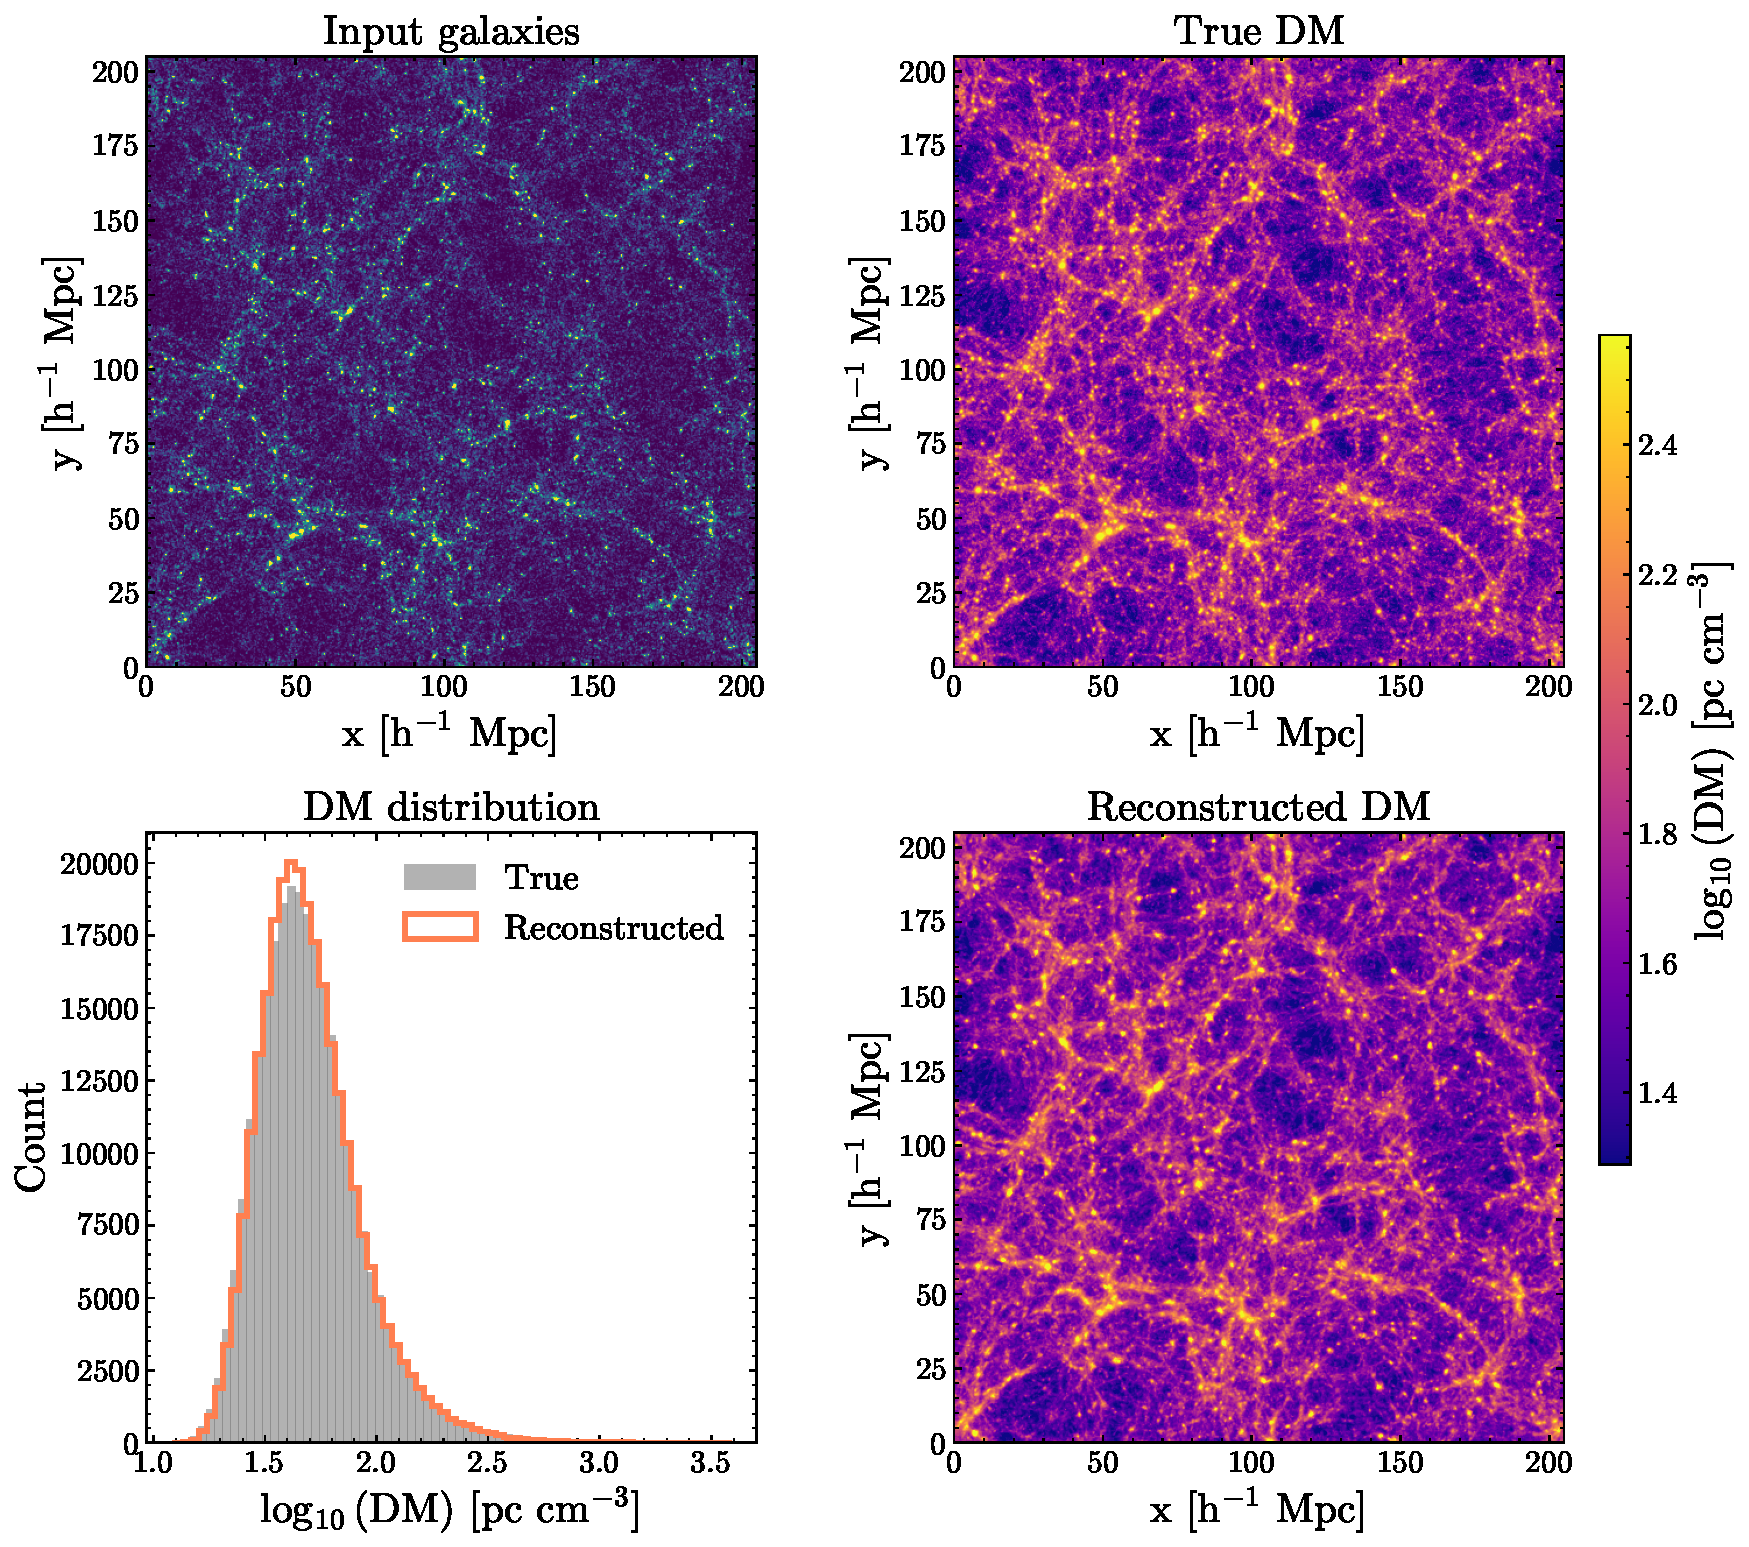
\includegraphics[width=0.5\linewidth]{figures/TNG300_generalization.pdf}
    \caption{\textbf{(Top left)} Input galaxy density field; \textbf{(top right)} true DM map from a TNG300 simulation box of size $(205\,h^{-1}\,\mathrm{Mpc})^3$; \textbf{(bottom right)} the model's reconstructed DM. The model was trained exclusively on CAMELS50 boxes of $(50\,h^{-1}\,\mathrm{Mpc})^3$, making this a 4$\times$ scaling test. \textbf{(Bottom left)} Histogram comparing the distribution of true DM values (gray) to reconstructed DM values (orange) across the entire TNG300 box. The reconstructed DM has been rescaled to match the median of the true DM, correcting an overall $\sim0.1$ dex underprediction by the model, after which the two distributions closely agree.
}
    \label{fig:tng300}
  \end{figure*}
}

\newcommand{\figCigar}{%
  \begin{figure*}
    \centering
    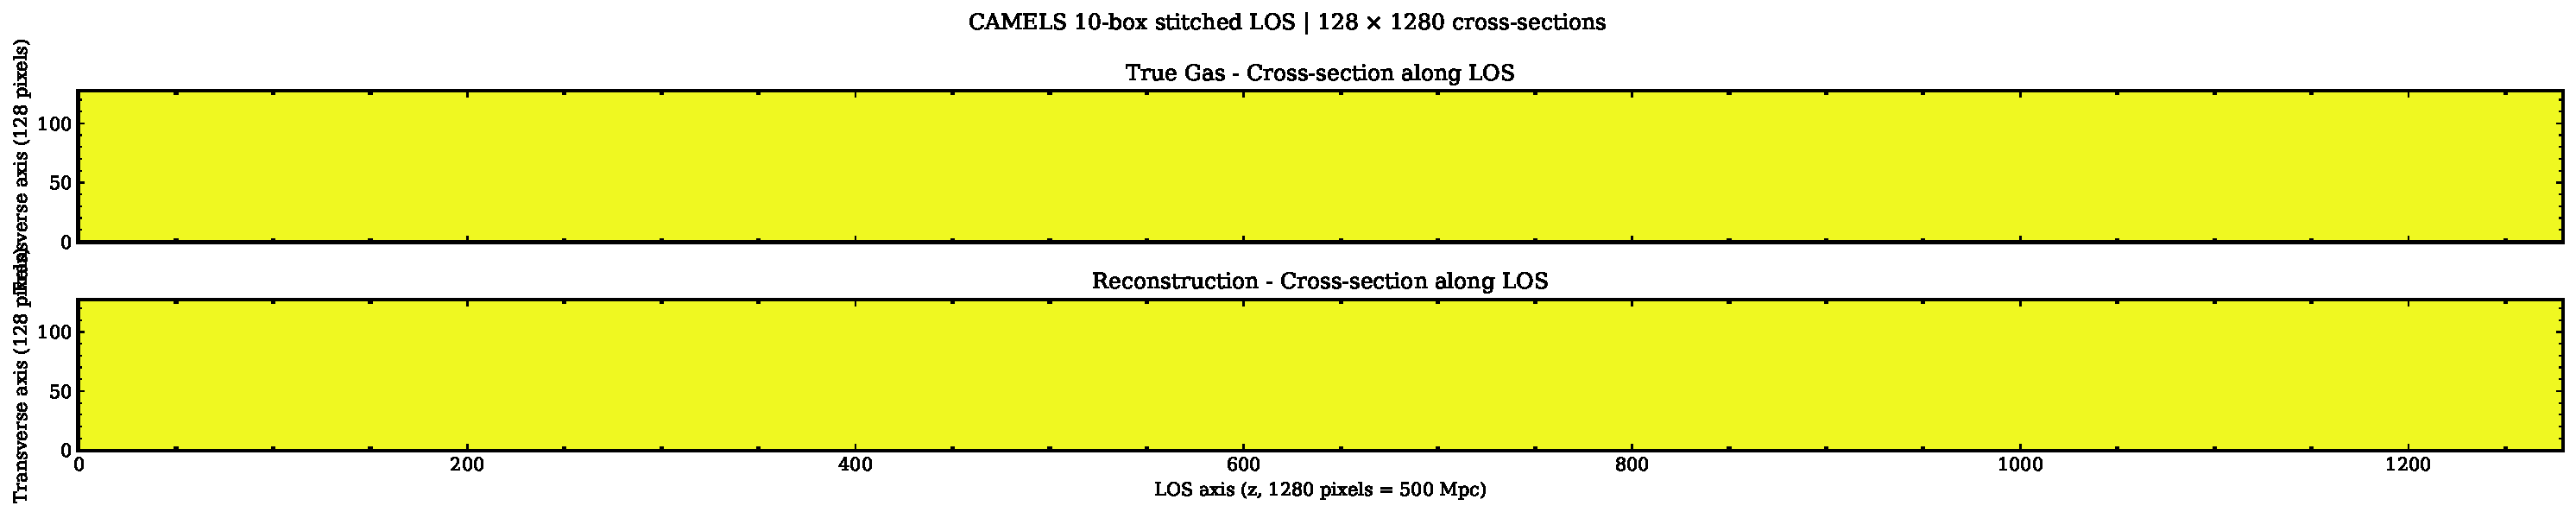
\includegraphics[width=0.98\linewidth]{figures/stitched_boxes.pdf}
    \caption{An example of a reconstructed FRB line of sight on simulated data. 10 CAMELS50 simulation boxes are tiled along the line-of-sight axis to construct an extended sightline spanning $\sim500\,h^{-1}\,\mathrm{Mpc}$. \textbf{Top:} True gas density field from the simulation. \textbf{Bottom:} Model reconstruction of the gas density field; the white dashed line marks an example FRB sightline, with the source location indicated by the star. The model successfully recovers the large-scale gas structure across the full stitched volume, demonstrating its ability to reconstruct realistic FRB sightlines from galaxy observations alone.}
    \label{fig:cigar}
  \end{figure*}
}

\newcommand{\figModelComparison}{%
  \begin{figure*}
    \centering
    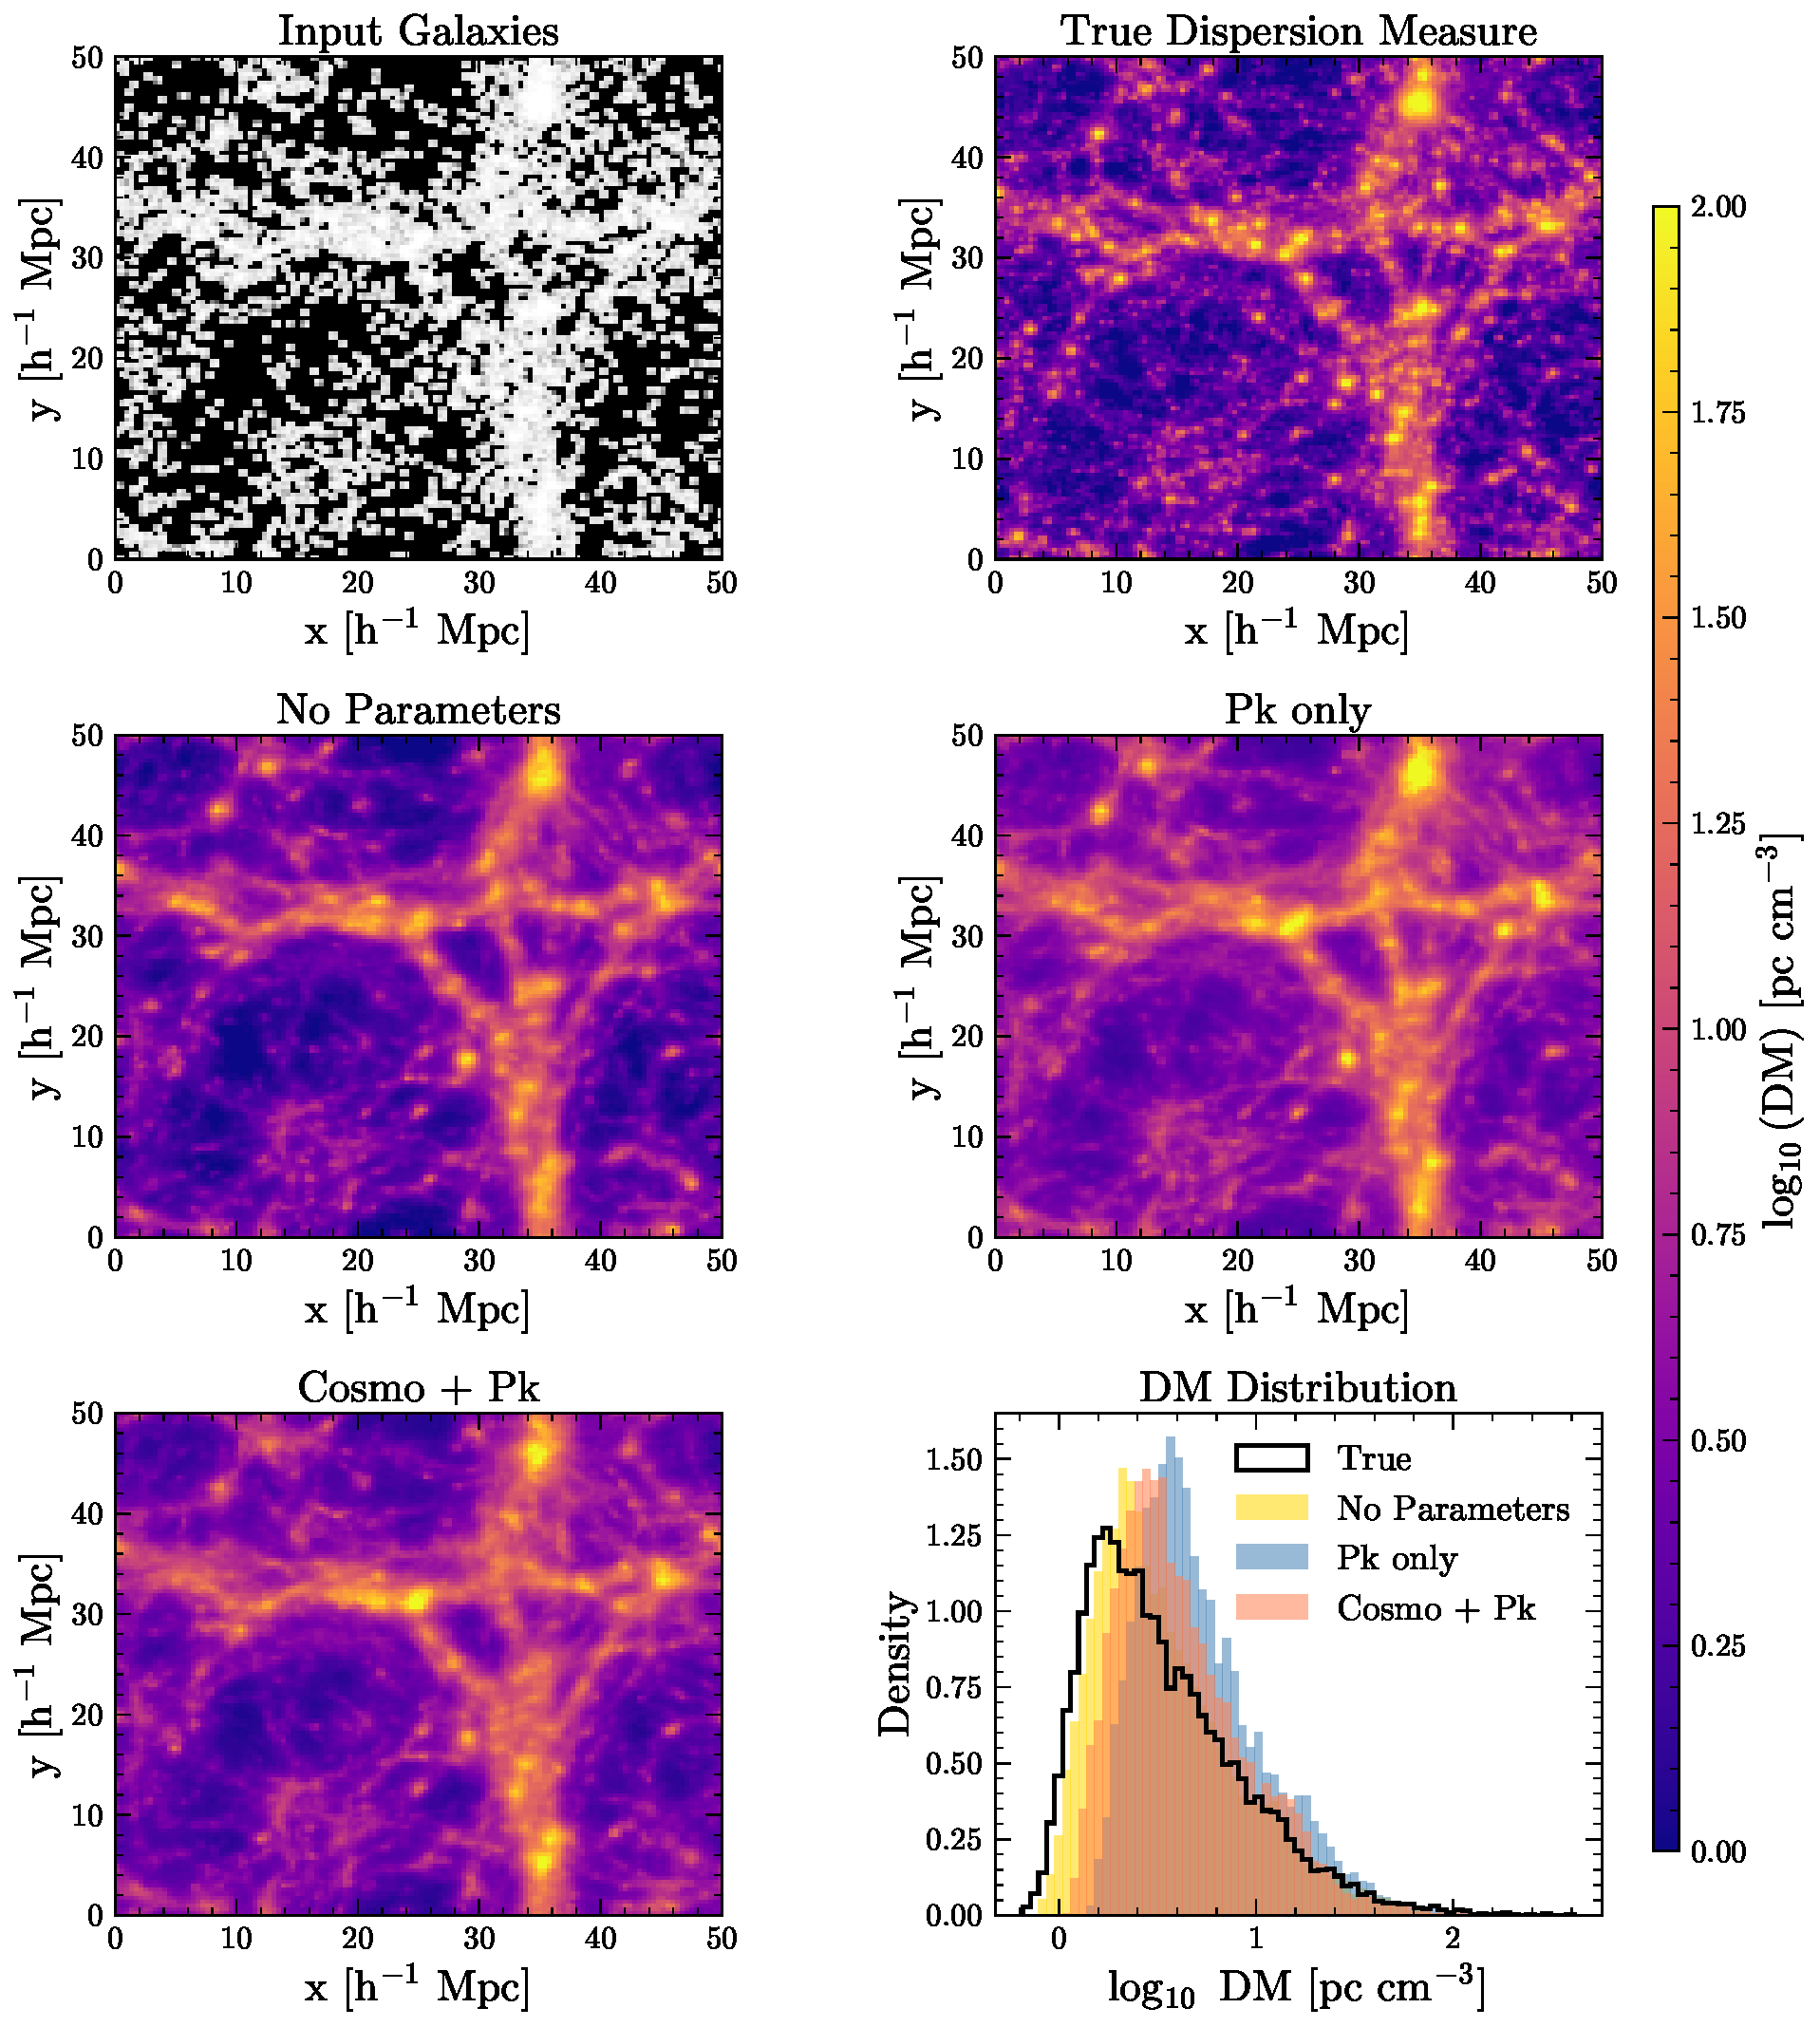
\includegraphics[width=0.5\linewidth]{figures/model_comparison.pdf}
    \caption{$(M_\odot/h)/({\rm Mpc}/h)^3$Input galaxy density field; true DM map; reconstructed DM from three different models that condition on cosmology in different ways. The three models are: (1) conditioning on the baryonic suppression power spectrum (`cosmo normalization pk`), (2) conditioning on 11 selected cosmological parameters (`params maryam`), and (3) a baseline model that does not condition on cosmological parameters at all (`marginalized`). Histogram comparing the DM distributions produced by each model (colored) to the true distribution (black line).
}
    \label{fig:model_comparison}
  \end{figure*}
}

\newcommand{\figRank}{%
  \begin{figure*}
    \centering
    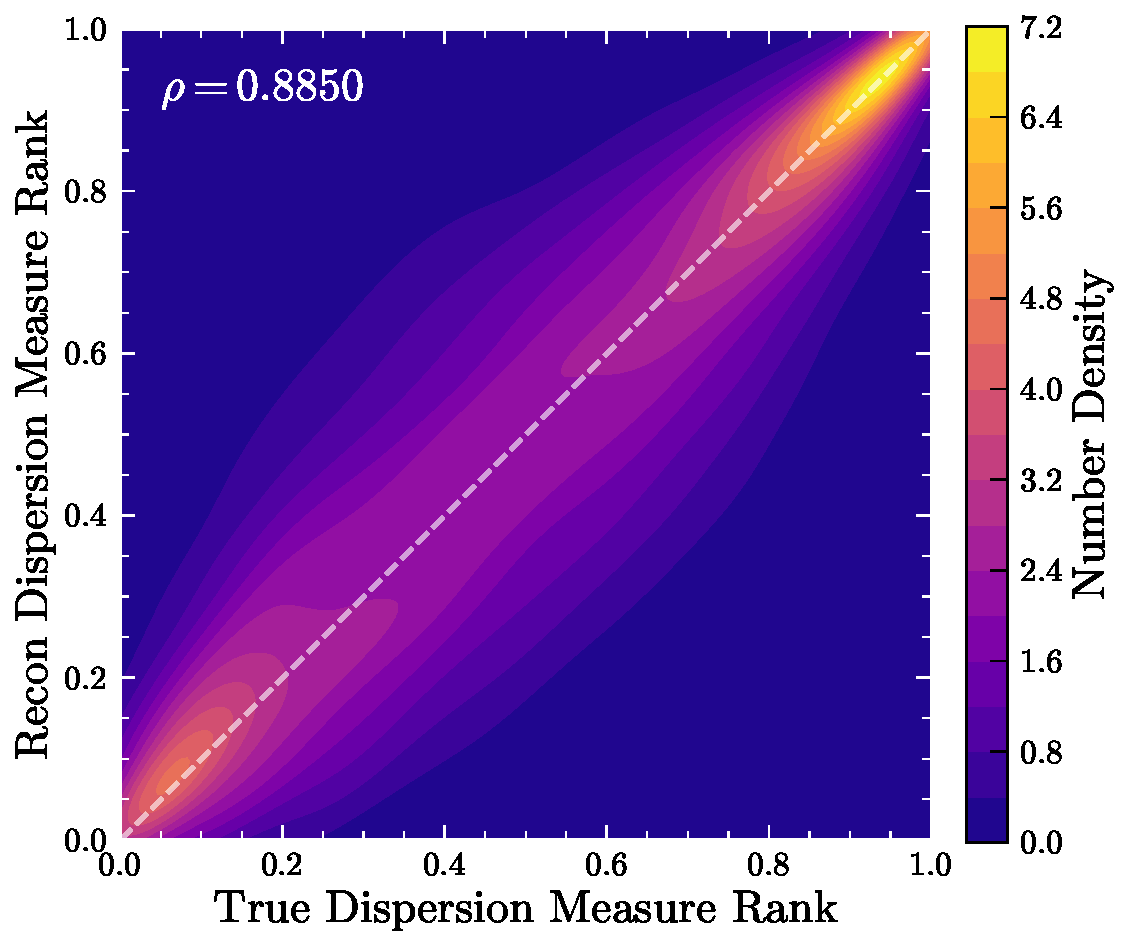
\includegraphics[width=0.5\linewidth]{figures/rank_density.pdf}
     \caption{
    2D histogram comparing the rank of true DM values (x-axis) to the rank of reconstructed DM values from the model's posterior mean (y-axis), with both axes normalized to $[0, 1]$. The white dashed line indicates perfect 1:1 agreement. The color scale (purple to yellow) shows the number density of lines of sight at each rank pair. The concentration of points along the diagonal demonstrates that the model preserves the relative ordering of DM values across the full dynamic range, even where absolute predictions may deviate. The Spearman rank correlation is $\rho = 0.8850$.
}
    \label{fig:rank}
  \end{figure*}
}
